%  article.tex (Version 3.3, released 19 January 2008)
%  Article to demonstrate format for SPIE Proceedings
%  Special instructions are included in this file after the
%  symbol %>>>>
%  Numerous commands are commented out, but included to show how
%  to effect various options, e.g., to print page numbers, etc.
%  This LaTeX source file is composed for LaTeX2e.

%  The following commands have been added in the SPIE class 
%  file (spie.cls) and will not be understood in other classes:
%  \supit{}, \authorinfo{}, \skiplinehalf, \keywords{}
%  The bibliography style file is called spiebib.bst, 
%  which replaces the standard style unstr.bst.  

\documentclass[]{spie}  %>>> use for US letter paper
%%\documentclass[a4paper]{spie}  %>>> use this instead for A4 paper
%%\documentclass[nocompress]{spie}  %>>> to avoid compression of citations
%% \addtolength{\voffset}{9mm}   %>>> moves text field down
%% \renewcommand{\baselinestretch}{1.65}   %>>> 1.65 for double spacing, 1.25 for 1.5 spacing 
%  The following command loads a graphics package to include images 
%  in the document. It may be necessary to specify a DVI driver option,
%  e.g., [dvips], but that may be inappropriate for some LaTeX 
%  installations. 
\usepackage[]{graphicx}
\usepackage{subfigure}
\usepackage{amsmath}
\usepackage{hyperref}
\usepackage{wrapfig}

\graphicspath{{images/}}

\title{SVA: Shape variation analyzer} 

%>>>> The author is responsible for formatting the 
%  author list and their institutions.  Use  \skiplinehalf 
%  to separate author list from addresses and between each address.
%  The correspondence between each author and his/her address
%  can be indicated with a superscript in italics, 
%  which is easily obtained with \supit{}.

\author{Priscille de Dumast\supit{a}, Clement Mirabel\supit{a}, Beatriz Paniagua\supit{b}, Marilia Yatabe\supit{a}, Antonio Ruellas,\supit{a}
Nina Tubau\supit{a}, Martin Styner\supit{c}, Lucia Cevidanes\supit{a}, Juan C. Prieto\supit{c}
\skiplinehalf
\supit{a}University of Michigan, Ann Arbor, United States \\
\supit{b}Kitware, Carrboro, United States; \\
\supit{c}University of North Carolina, Chapel Hill, United States;
}

%>>>> Further information about the authors, other than their 
%  institution and addresses, should be included as a footnote, 
%  which is facilitated by the \authorinfo{} command.

%%\authorinfo{Further author information: (Send correspondence to J.C.P.)}
%%>>>> when using amstex, you need to use @@ instead of @
 

%%%%%%%%%%%%%%%%%%%%%%%%%%%%%%%%%%%%%%%%%%%%%%%%%%%%%%%%%%%%% 
%>>>> uncomment following for page numbers
% \pagestyle{plain}    
%>>>> uncomment following to start page numbering at 301 
%\setcounter{page}{301} 
 
  \begin{document} 
  \maketitle 

%%%%%%%%%%%%%%%%%%%%%%%%%%%%%%%%%%%%%%%%%%%%%%%%%%%%%%%%%%%%% 
\begin{abstract}

Temporo-mandibular osteo arthritis (TMJ OA)
is characterized by progressive cartilage degradation and subchondral bone remodeling. The causes of this pathology remain 
unclear. Current research efforts are concentrated in finding new biomarkers
that will help us understand disease progression and ultimately improve the treatment of the disease. 
In this work, we present Shape Variation Analyzer (SVA), the goal is to develop a noninvasive technique to provide information about shape changes in TMJ OA. 
SVA uses neural networks to classify morphological variations of 3D models of the mandibular condyle. 
The shape features used for training include normal vectors, curvature and distances to average models of the condyles. 
The selected features are purely geometric and are shown to favor the classification task into 6 groups 
generated by consensus between two clinician experts. 
With this new approach, we were able to accurately classify 3D models of condyles. 
In this paper, we present the methods used and the results obtained with this new tool. 

\end{abstract}

%>>>> Include a list of keywords after the abstract 

\keywords{Temporo-mandibular osteo arthritis, deep learning, classification, artificial intelligence}

%%%%%%%%%%%%%%%%%%%%%%%%%%%%%%%%%%%%%%%%%%%%%%%%%%%%%%%%%%%%%
\section{INTRODUCTION}
\label{sec:intro}  % \label{} allows reference to this section

Osteoarthritis (OA), the most prevalent arthritis worldwide, is associated with significant pain and disability and affects 15\% of adults at any given time \cite{kalladka2014temporomandibular}. 

\begin{wrapfigure}{r}{0.35\textwidth}
    \centering
    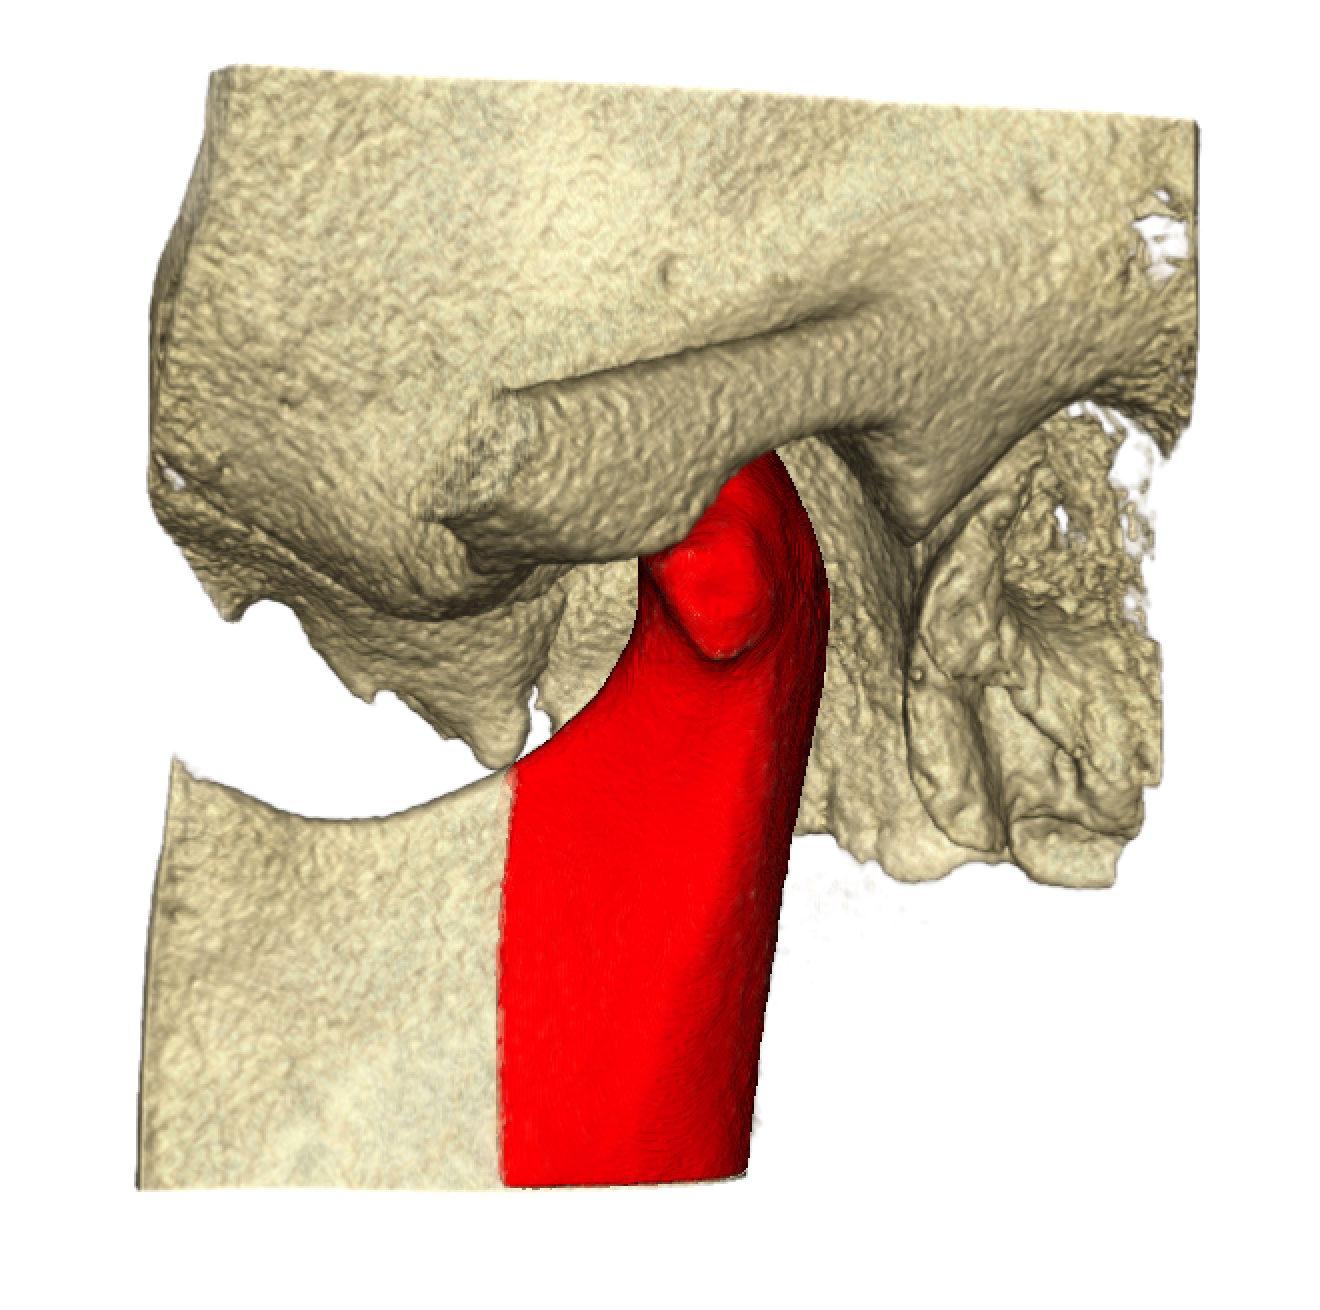
\includegraphics[width=0.3\textwidth]{mandibular-condyles.png}
    \caption{Volume rendering of CT image. Mandibular condyles in red.}
    \label{fig:mandibular}
\end{wrapfigure}
The complex pathogenesis of temporomandibular joint (TMJ) OA remains unclear to this day, and understanding its progression challenges experts given the different morphological patterns of bone resorption and formation observed in its various stages. The disease may evolve into repair and morphological adaptation, but also into aggressive bone destruction and functional impairment. 
Patients with OA present a variety of symptoms including pain, limited jaw movement, grinding, clicking, 
and deviation on opening.
Figure \ref{fig:mandibular} shows the mandibular condyles. 
There is no method to quantify morphology for early diagnosis, assessment of disease progression and treatment effects. 
The symptoms are different from patient to patient, i.e., TMJ OA may be in a quiet state until is set of by an array 
of events, or it may be painful from the start. However, recent work quantifying condylar morphology revealed 
differences between OA and asymptomatic condyles\cite{cevidanes2010quantification}.

The goal of this work is to develop a noninvasive technique to provide information about bony changes and disease changing in TMJ OA, using shape analysis. 
Given the complexity of such heterogeneous conditions and current clinical, biological, and imaging data in arthritis of the temporomandibular joint, there is a compelling need for more efficient software tools to facilitate these analyses. To answer this challenge, we developed Shape Variation Analyzer (SVA) using a neural network to classify morphological variations using 3D models of the mandibular condyle. In this work, we created 7 different categories for the classification task: 0. Normal, 1. Overgrowth, 2. Close to Normal, 3. Degeneration 1, 4. Degeneration 2, 5. Degeneration 3, 6. Degeneration 4; Figure \ref{fig:shapeGroups} shows samples of each group with the average shape of the control group. 

\begin{figure}
\centering 
    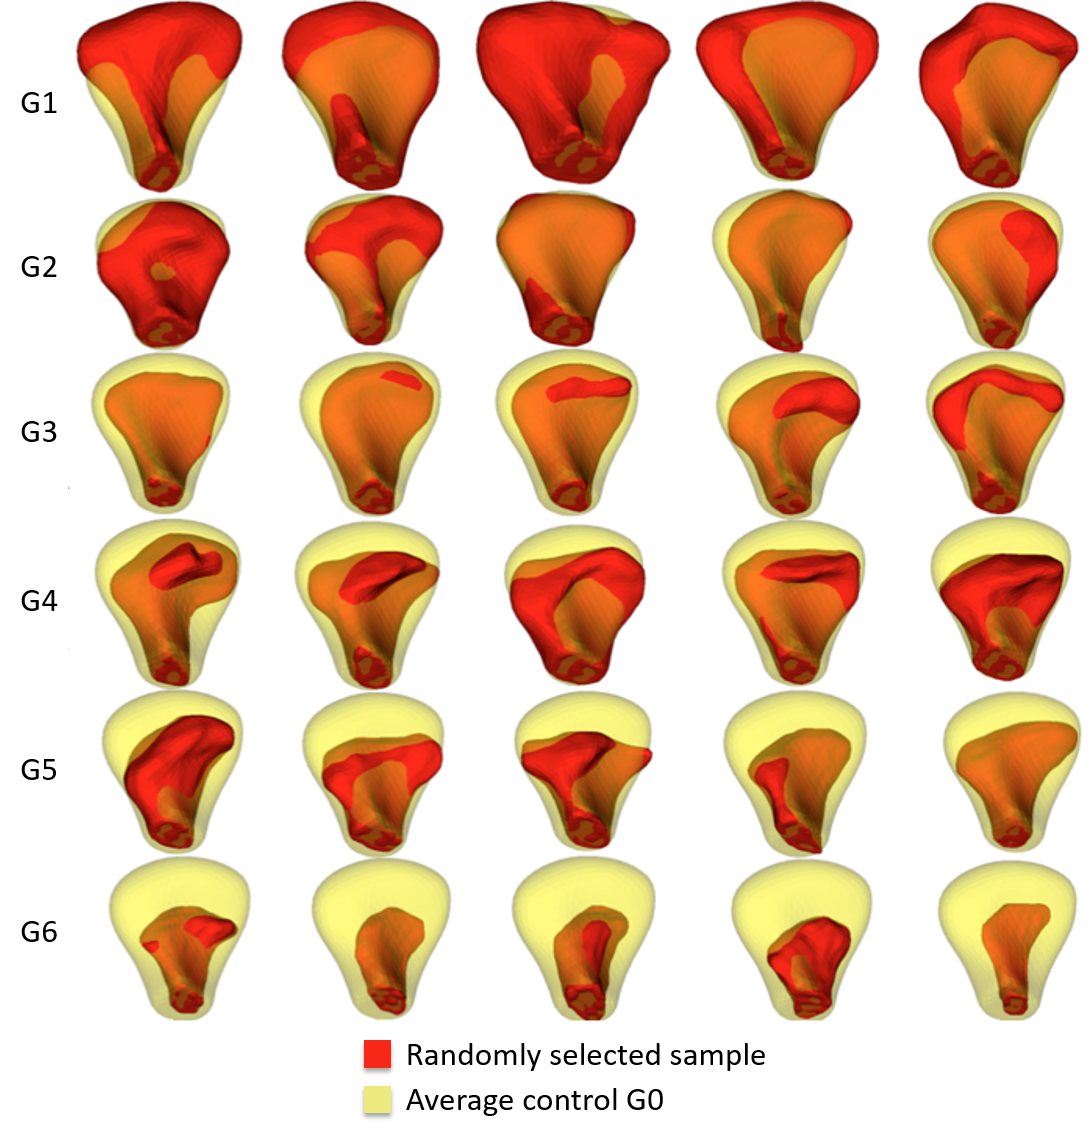
\includegraphics[width=0.95\textwidth]{ShapeGroupsSVA.png}
    \caption{Randomly selected subject samples for each group shown in red. In yellow, the average shape from the control group rendered transparent. G1. Overgrowth, G2. Close to Normal, G3. Degeneration 1, G4. Degeneration 2, G5. Degeneration 3, G6. Degeneration 4}
    \label{fig:shapeGroups}
\end{figure} 

The development of this tool did not consist only on building and training a neural network but also
the pre-processing steps to prepare the data, which include generating 3D models of the condyles \cite{PANIAGUA2011345}, improve shape correspondence \cite{lyu2013group}, and extract shape features from the 3D models. The process of extracting
shape features are detailed in this paper. 
The features are selected because they are purely geometric and they do not depend on the position 
nor the orientation of the model, which may vary across the different groups in the population, 
and may introduce bias for the analysis.

\section{MATERIALS}

The study group consists of 268 TMJ joints (163 TMJ OA, 105 asymptomatic controls), obtained from Cone Beam Computed Tomography (CBCT) scans (i-CAT Next Generation, $120 kV$, $18.66 mA$). TMJ OA joints were subdivided, by consensus between 2 clinicians, into 6 subgroups based in morphological variability, compared to the average control morphology.
Figure \ref{fig:condylesHisto} shows the distribution of samples across the different groups in TMJ OA.
\begin{figure}[h]
\centering 
    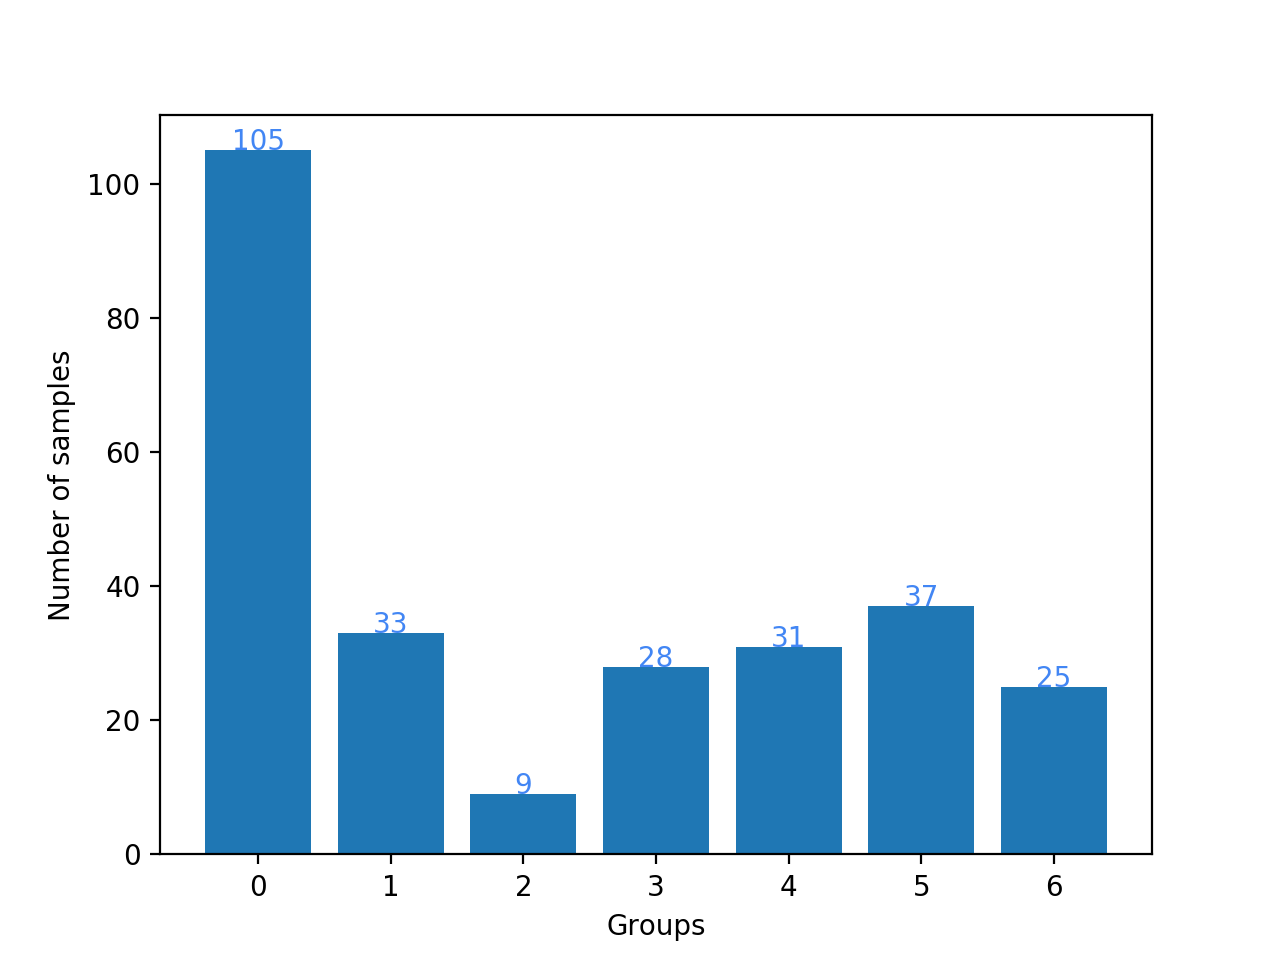
\includegraphics[width=0.6\textwidth]{NumberSamplesCondyles.png}
    \caption{Distribution of condyles in the different groups. G0. Control, G1. Overgrowth, G2. Close to Normal, G3. Degeneration 1, G4. Degeneration 2, G5. Degeneration 3, G6. Degeneration 4}
    \label{fig:condylesHisto}
\end{figure} 

%%%%%%%%%%%%%%%%%%%%%%%%%%%%%%%%%%%%%%%%%%%%%%%%%%%%%%%%%%%%%
\section{METHODS} 

\subsection{Model creation}

\begin{figure}
\centering 
    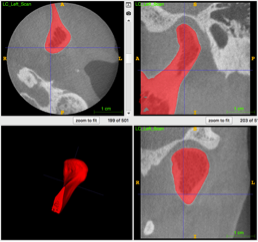
\includegraphics[width=0.7\textwidth]{ITKSnapCondyles.png}
    \caption{Manual segmentation of Condyles using ITK-SNAP}
    \label{fig:itkSnapCondyle}
\end{figure} 
\begin{figure}
\centering 
    \subfigure[]{\label{fig:result1_bi}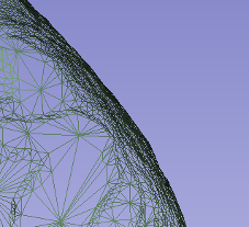
\includegraphics[width=0.35\textwidth]{MeshModelMaker-Wireframe.png}}
    \subfigure[]{\label{fig:result2_bi}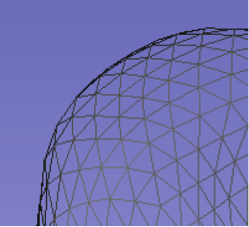
\includegraphics[width=0.35\textwidth]{MeshAfterSpharm.png}}
    \caption{Figure (a) shows a condylar model generated with marching cubes. Figure (b) shows a condylar model 
    after the parameterization via spherical harmonics. The tessellation is regular, i.e, equal area, and the models contain the same
    number of points across the population.}
    \label{fig:result_bi}
\end{figure} 

The CBCT images are segmented using a semi-automated method in ITK-SNAP\cite{py06nimg}. The software allows manual editing to clean the segmentation. Figure \ref{fig:itkSnapCondyle} shows a screen-shot of the application with different orthogonal slices
of the image.
Using EasyClip\footnote{https://www.slicer.org/wiki/Documentation/4.8/Extensions/EasyClip} (a module included in 3DSlicer), the condylar models are simultaneously cropped to define the condylar region of interest. The cropped segmentation maps are used to generated regular tessellations.

% \begin{figure}
% \centering 
%     \label{fig:modelMaker}
%     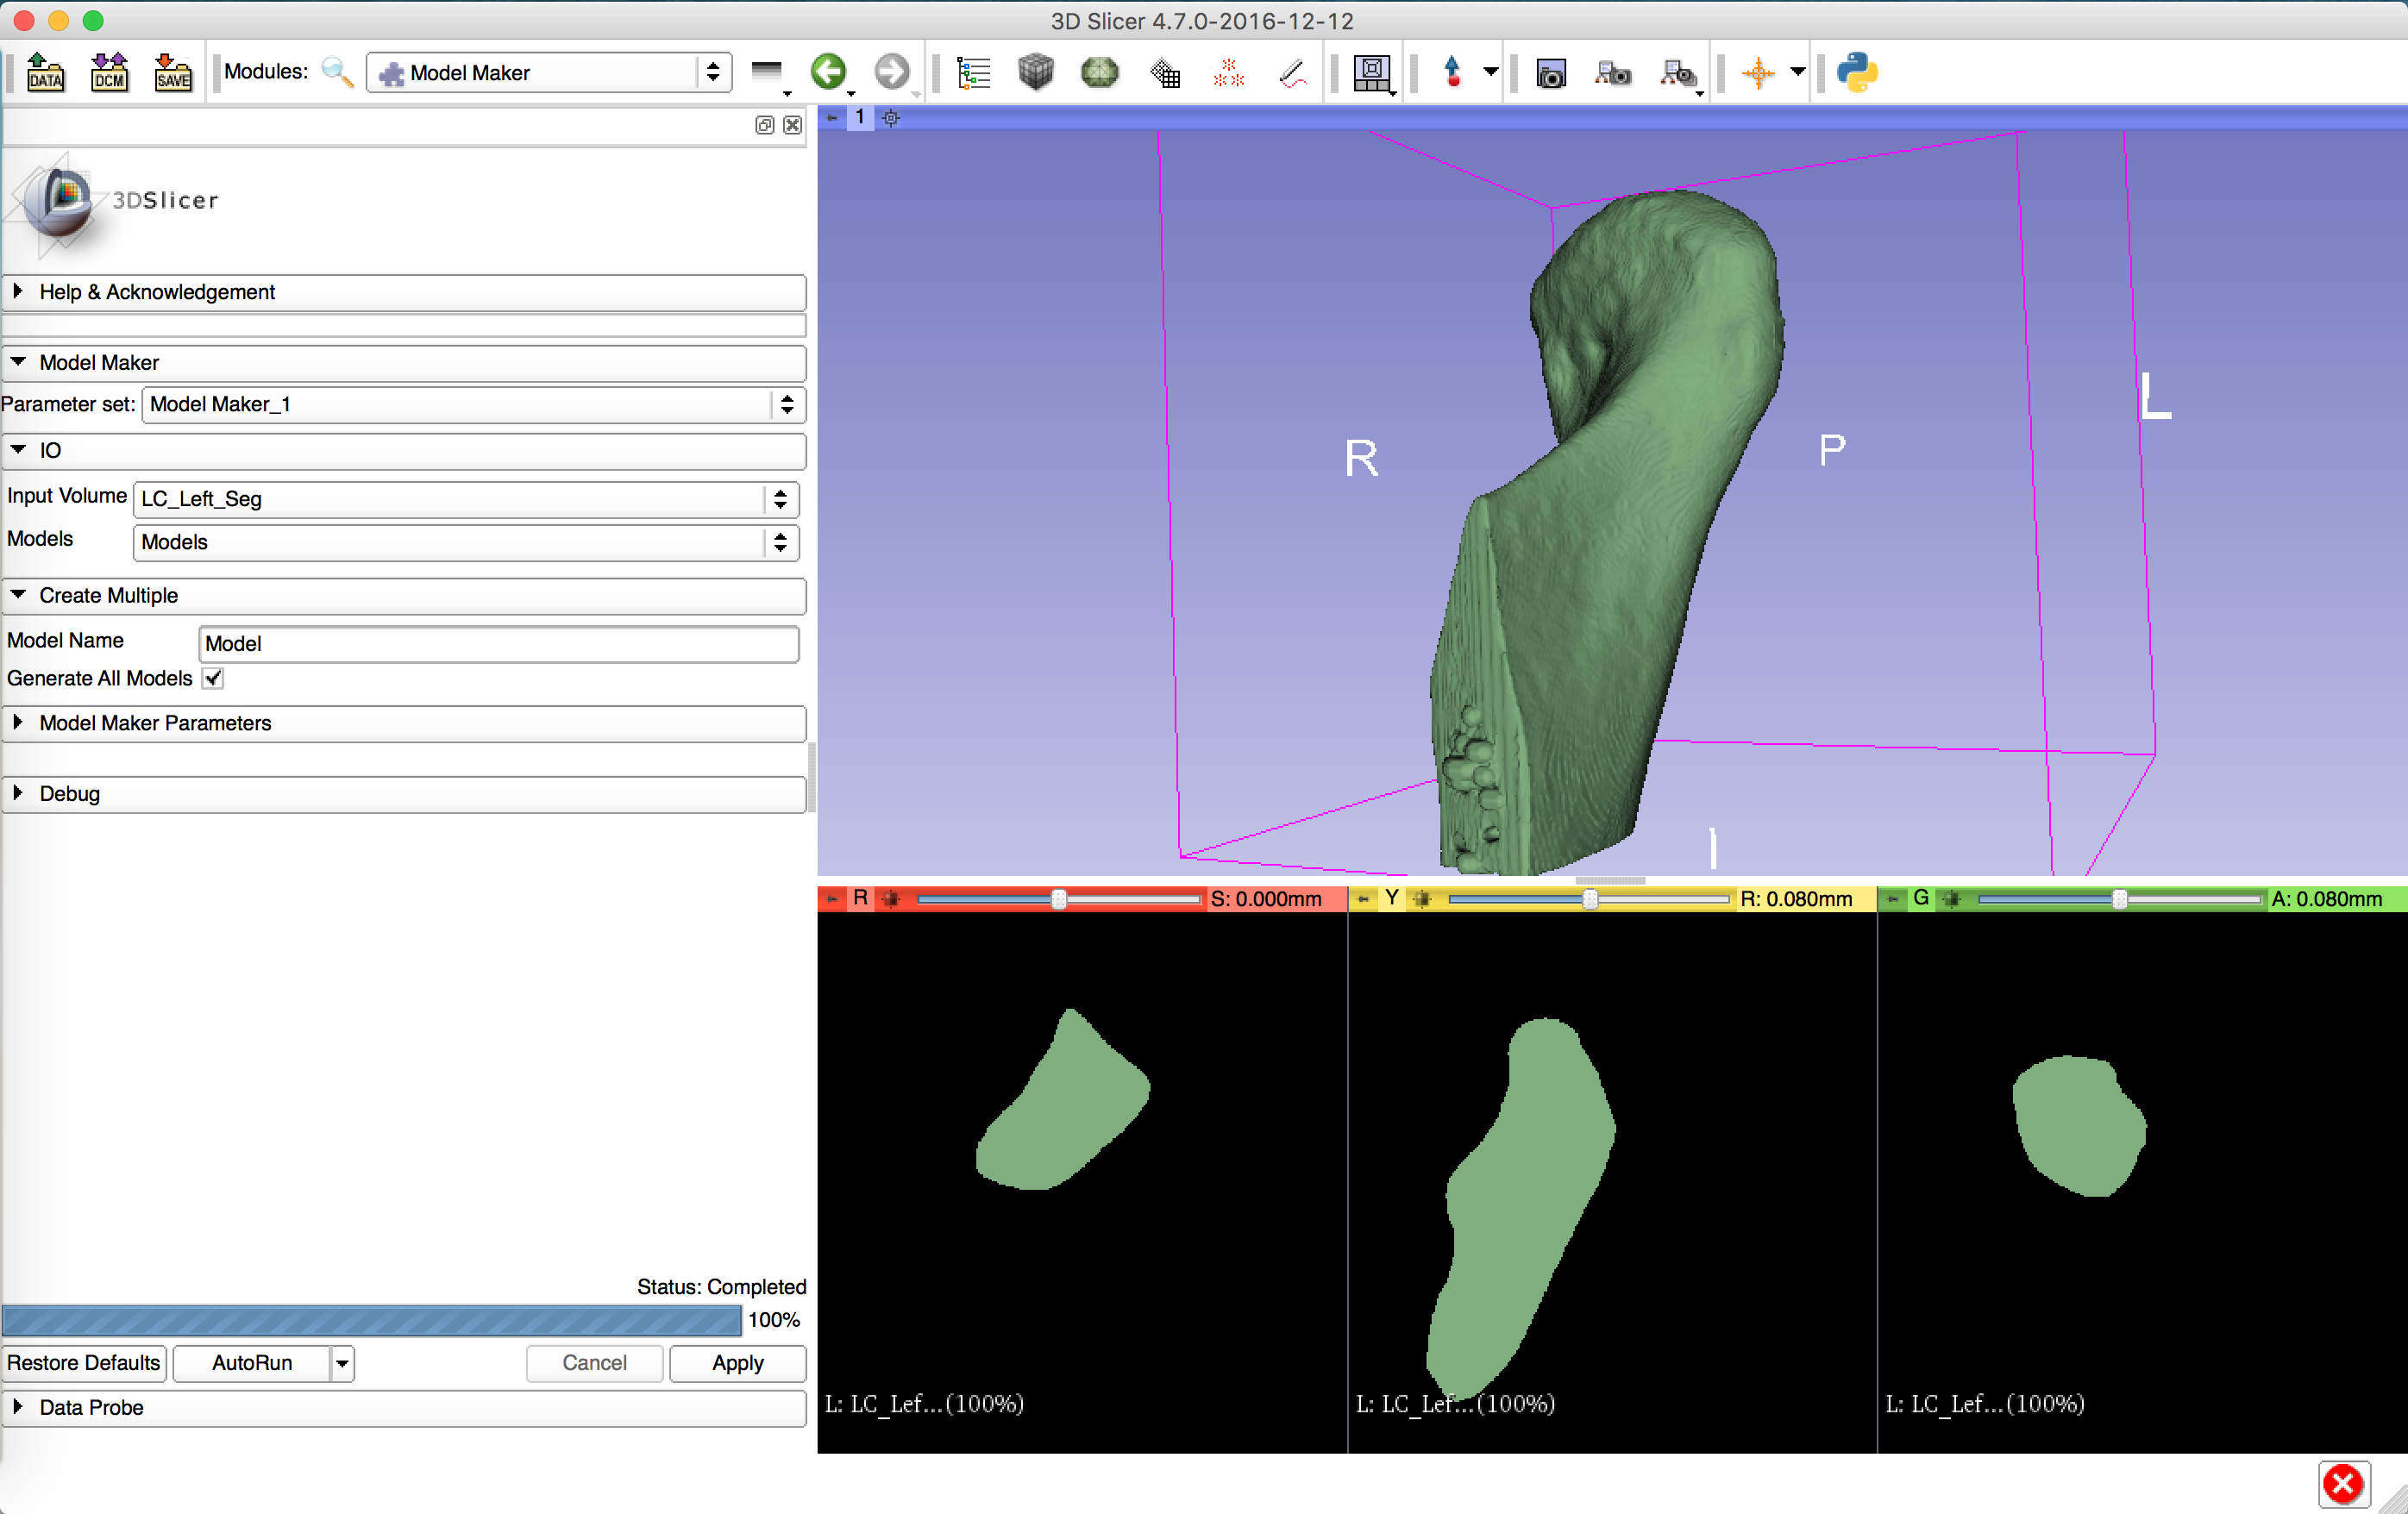
\includegraphics[width=0.25\textwidth]{ModelMaker-FullView.png}
%     \caption{The 3D model is used to define the condylar region of interest. Using the module EasyClip, the condylar models are simultaneously cropped. The cropped segmentation maps are used as input for SPHARM-PDM.}
% \end{figure}

Spherical harmonics representation point distributed models (SPHARM-PDM)\cite{styner2006framework} is used to generate a mesh with 1002 points, via spherical mapping and spherical parametrization of the input segmentation maps. 
SPHARM-PDM generates a regular mesh, as show in Figure \ref{fig:result1_bi}.
After the models have the same number of points and a regular mesh, we proceed to place landmarks in the 3D models. 
The landmarks are placed in homologous regions for all individuals. Figure \ref{fig:registration} shows a condyle 
with the landmarks placed on the surface. 
\begin{wrapfigure}{r}{0.35\textwidth}
    \centering
    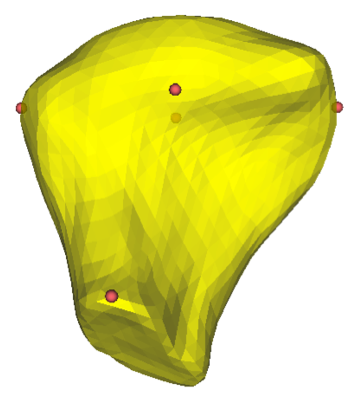
\includegraphics[width=0.3\textwidth]{LandmarksCondyle.png}
    \caption{Landmarks in red, displayed in the surface of a condyle 3D model.}
    \label{fig:registration}
\end{wrapfigure}
These landmarks are used to generate a tessellation with correspondent points 
employing a group-wise registration method\cite{lyu2013group}.
Figure \ref{fig:groups} shows the condylar models aligned where regions in the 3D model correspond across the population.

\begin{figure}[b]
\centering 
    \subfigure[]{\label{fig:RigidAlignmentBefore}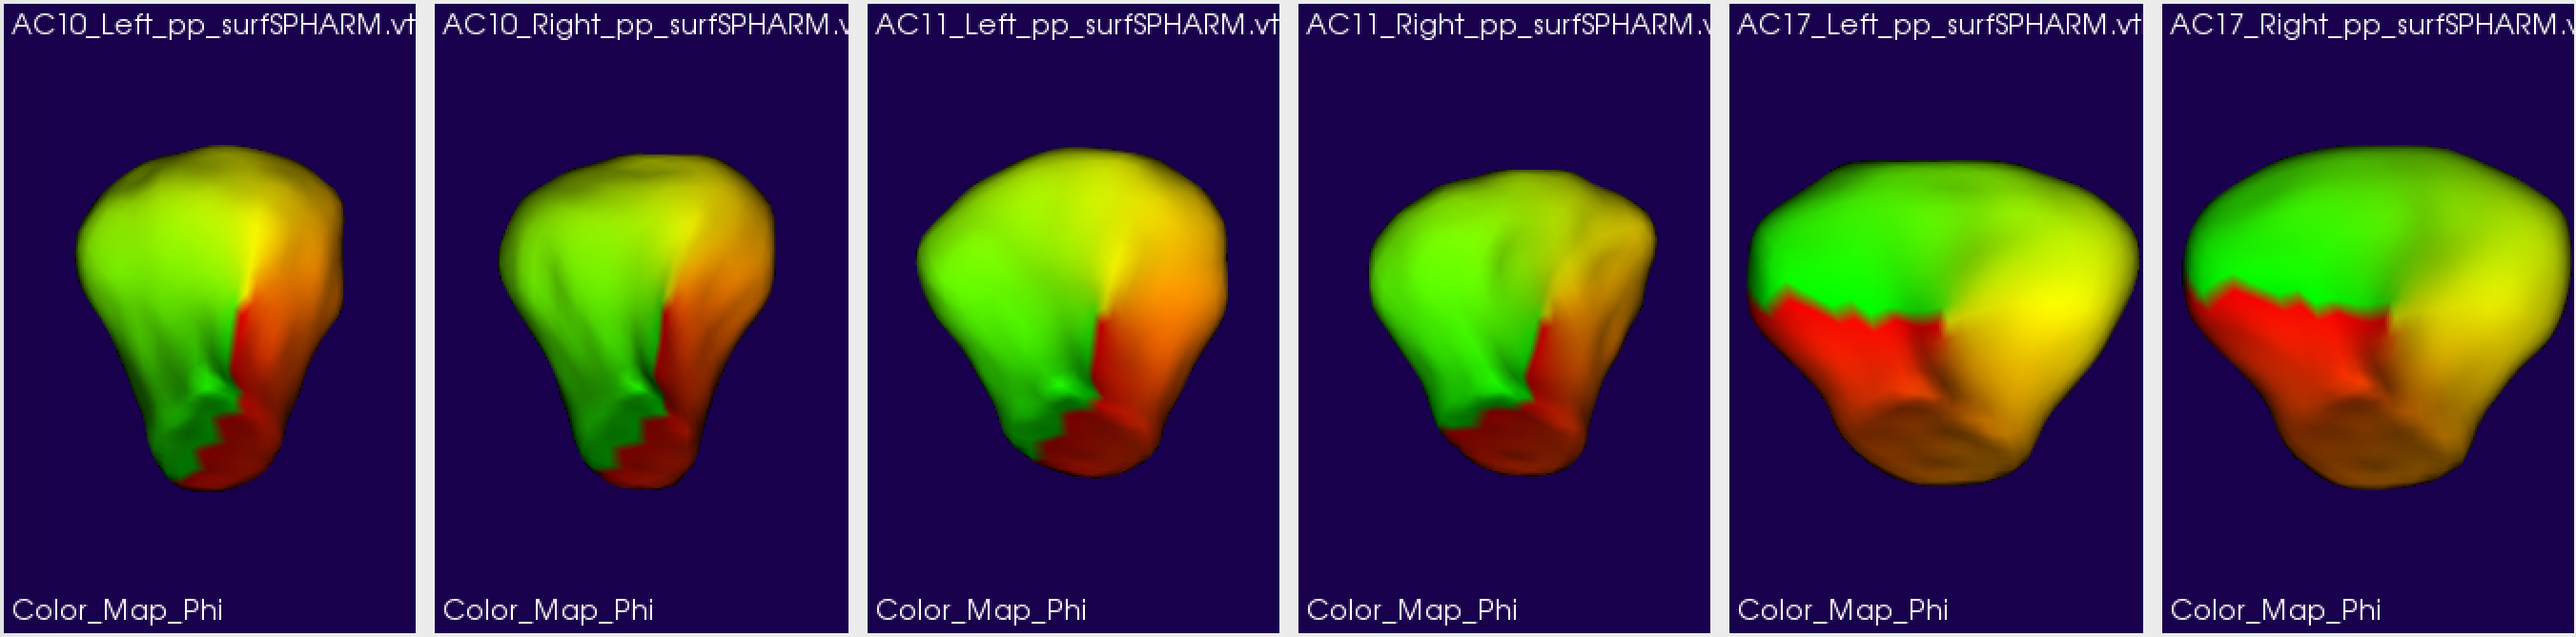
\includegraphics[width=0.95\textwidth]{RigidAlignment-before.png}}
    \subfigure[]{\label{fig:RigidAlignmentAfter}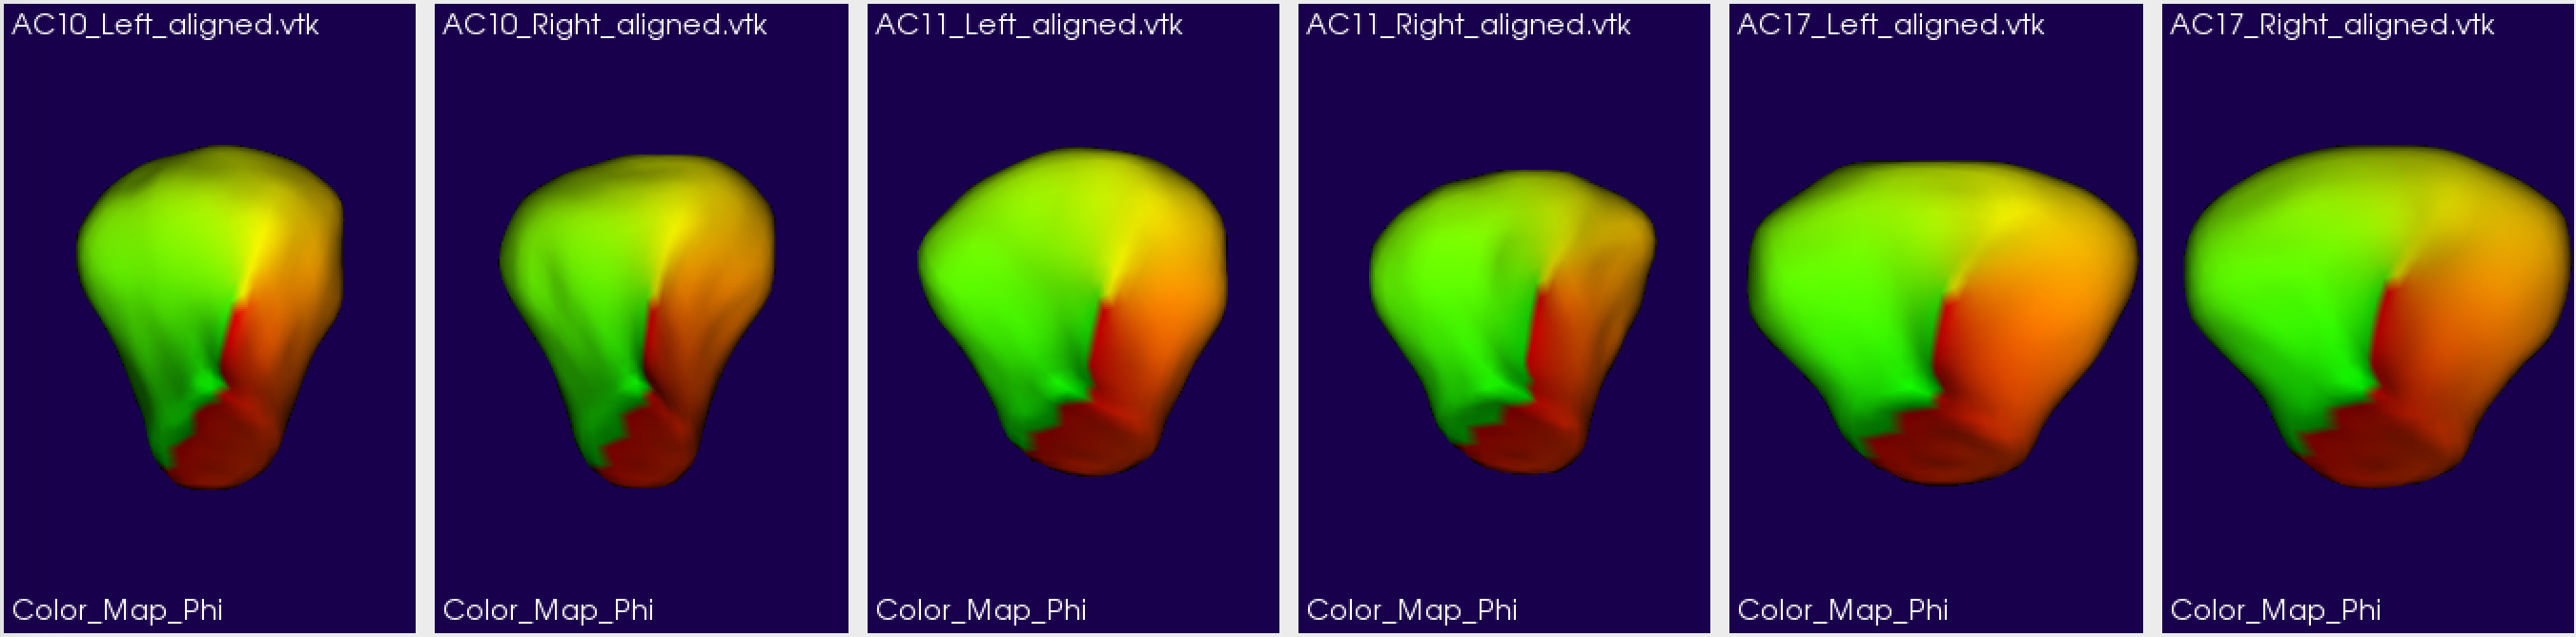
\includegraphics[width=0.95\textwidth]{RigidAlignment-after.png}}
    \caption{Group-wise correspondence (GROUPS). Figure (a) shows the models generated by SPHARM-PDM. The spherical parameterization produced by SPHARM and the landmarks are used to generate 3D models that have correspondent points across subjects. The rainbow color map in the 3D models encode the location. Figure (b) shows the 3D models after GROUPS processing, similar colors are found at every point in the model across all the samples 
    in the population.}
    \label{fig:groups}
\end{figure}

\subsection{Feature extraction}

Using the aligned 3D models, an average model is created for each group.
The features that led to higher accuracy in classification include 
the normal vectors, mean curvature of the surface, and the distances to the average meshes. 
In general, the input data for our network has shape  $N * n_{pt} * n_{feat}$ where $N$ is the batch size during training, 
$n_{pt} = 1002$ and $n_{feat} = 10$. These features do not include any information about position and are purely geometric.

\begin{figure}[t]
\centering 
    \subfigure[Mean curvature]{\label{fig:feat1}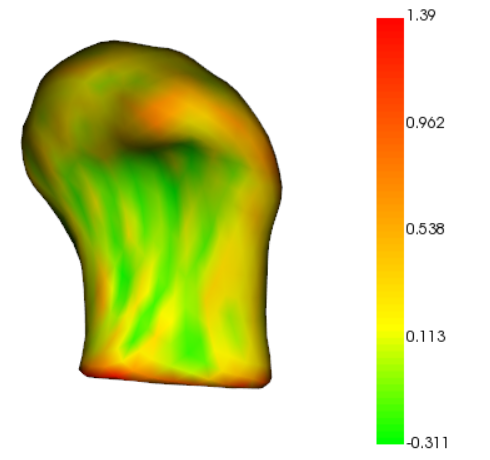
\includegraphics[width=0.35\textwidth]{MeanCurvatureSVA.PNG}}
    \subfigure[Normal vectors]{\label{fig:feat2}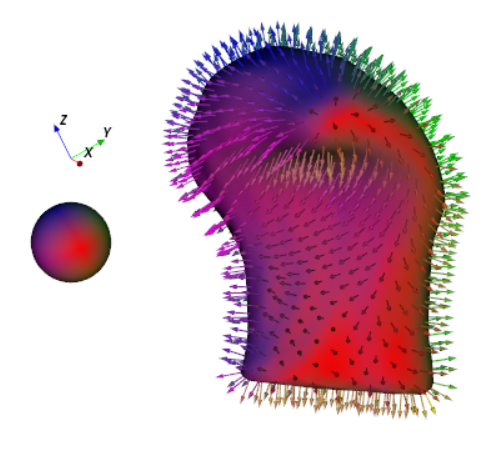
\includegraphics[width=0.35\textwidth]{NormalsSVA.PNG}}\\
    \subfigure[G1]{\label{fig:feat3}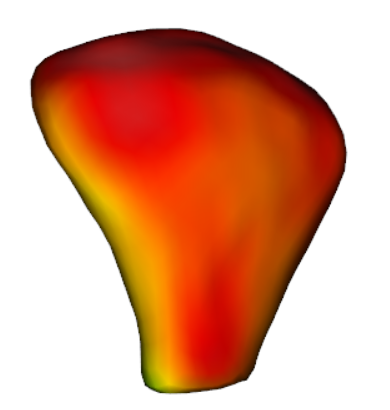
\includegraphics[width=0.14\textwidth]{DistanceG1SVA.PNG}}
    \subfigure[G2]{\label{fig:feat4}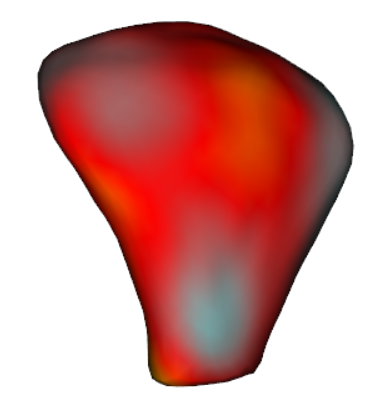
\includegraphics[width=0.14\textwidth]{DistanceG2SVA.PNG}}
    \subfigure[G3]{\label{fig:feat5}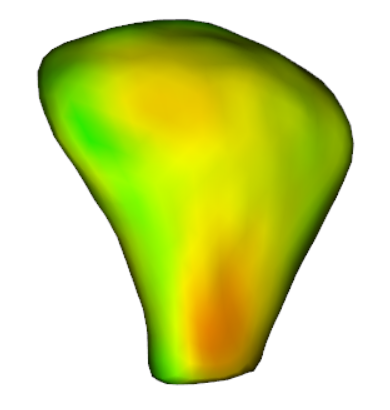
\includegraphics[width=0.14\textwidth]{DistanceG3SVA.PNG}}
    \subfigure[G4]{\label{fig:feat6}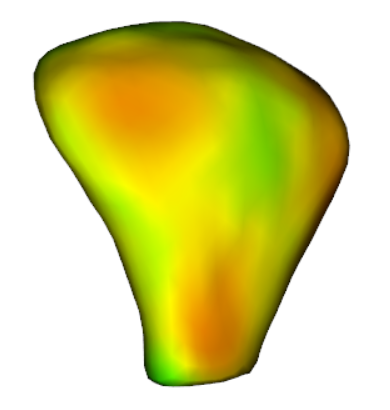
\includegraphics[width=0.14\textwidth]{DistanceG4SVA.PNG}}
    \subfigure[G5]{\label{fig:feat7}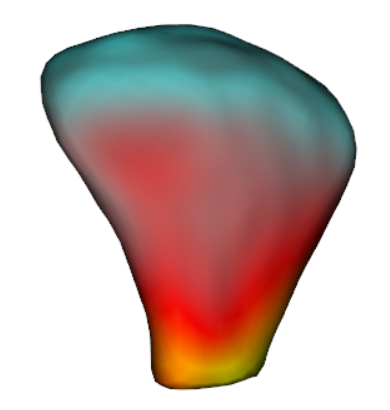
\includegraphics[width=0.14\textwidth]{DistanceG5SVA.PNG}}
    \subfigure[G6]{\label{fig:feat8}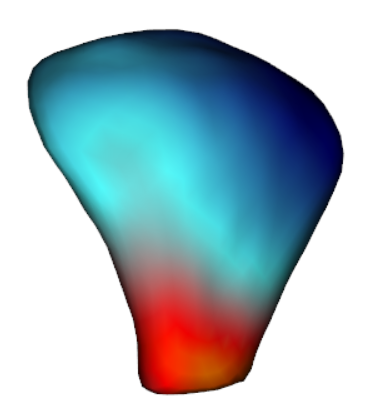
\includegraphics[width=0.14\textwidth]{DistanceG6SVA.PNG}}
    \subfigure{\label{fig:feat8}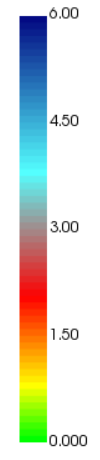
\includegraphics[width=0.04\textwidth]{DistanceColorBarSVA.PNG}}
    \caption{Visualization of the features computed for every condyle model at every point. Figure (a) shows the mean curvature of a model. Figure (b) shows normal vectors, color coded for direction. Figures (c)-(h) show color coded distance of every point to the average model of that particular group. In total the number of features is 10 for every point in the model.}
    \label{fig:svafeatures}
\end{figure} 
Figure \ref{fig:svafeatures} shows the different features computed for every model in the population.
As shown in Figure \ref{fig:condylesHisto}, the groups have a significant difference in the number of samples, i.e., 
an imbalanced dataset.
Training a neural network with an imbalanced dataset is known as the class imbalance problem \cite{japkowicz2002class}.
If a neural network is trained with an imbalanced dataset, it will learn to identify the majority class
more often. In order to have a balance dataset, we use a synthetic minority over-sampling technique (SMOTE)\cite{chawla2002smote}.

\begin{figure}[h]
\centering 
    \subfigure[Principal component analysis (PCA) of the original dataset (268). 89 components are necessary to explain $95\%$ of the variance.]{\label{fig:SMOTEresample_pca}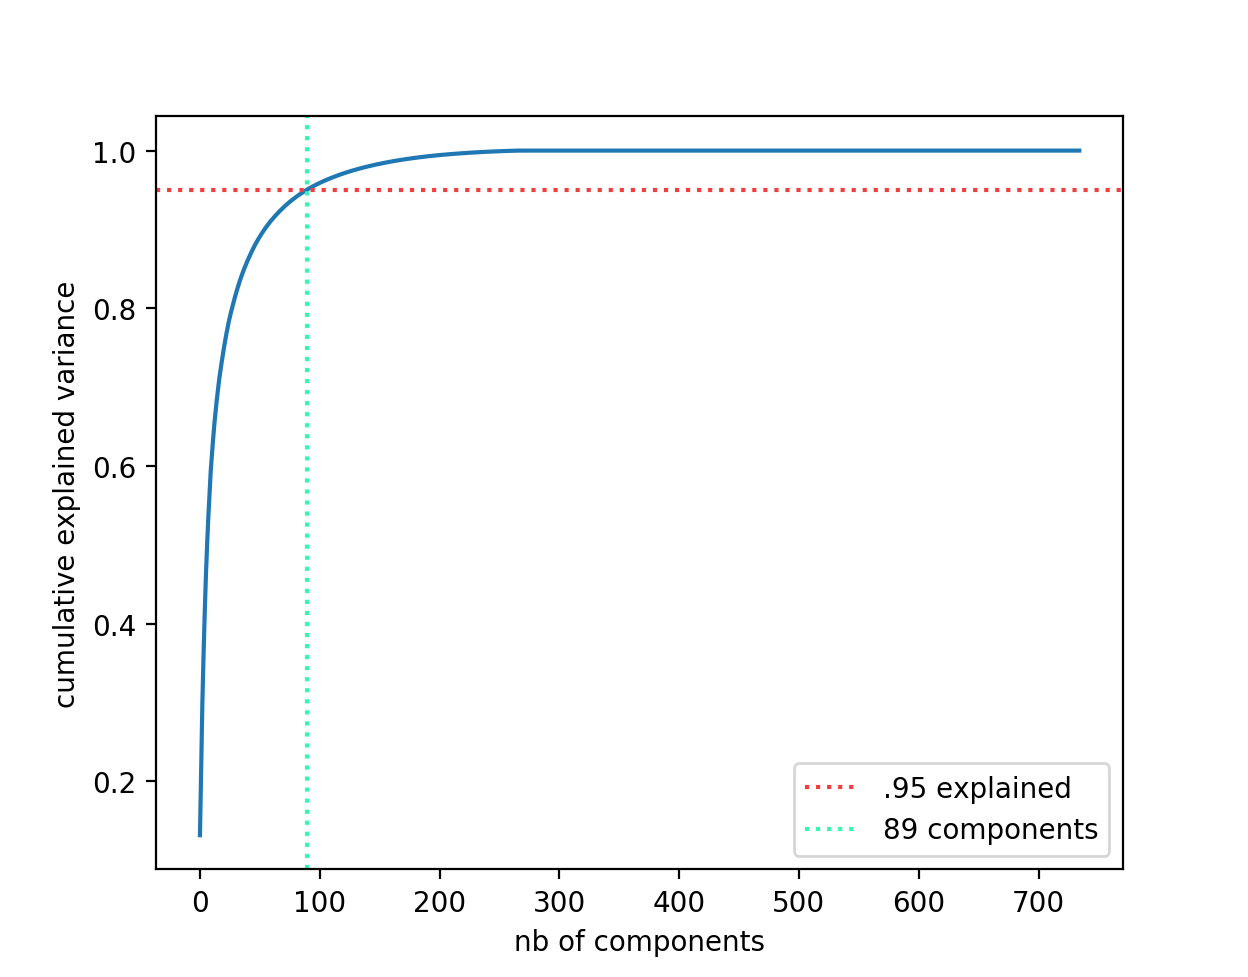
\includegraphics[width=0.45\textwidth]{pca_explained.png}}
    \subfigure[SMOTE on feature space. The first two principal components are used to plot the datasets.]{\label{fig:SMOTEresample_smote}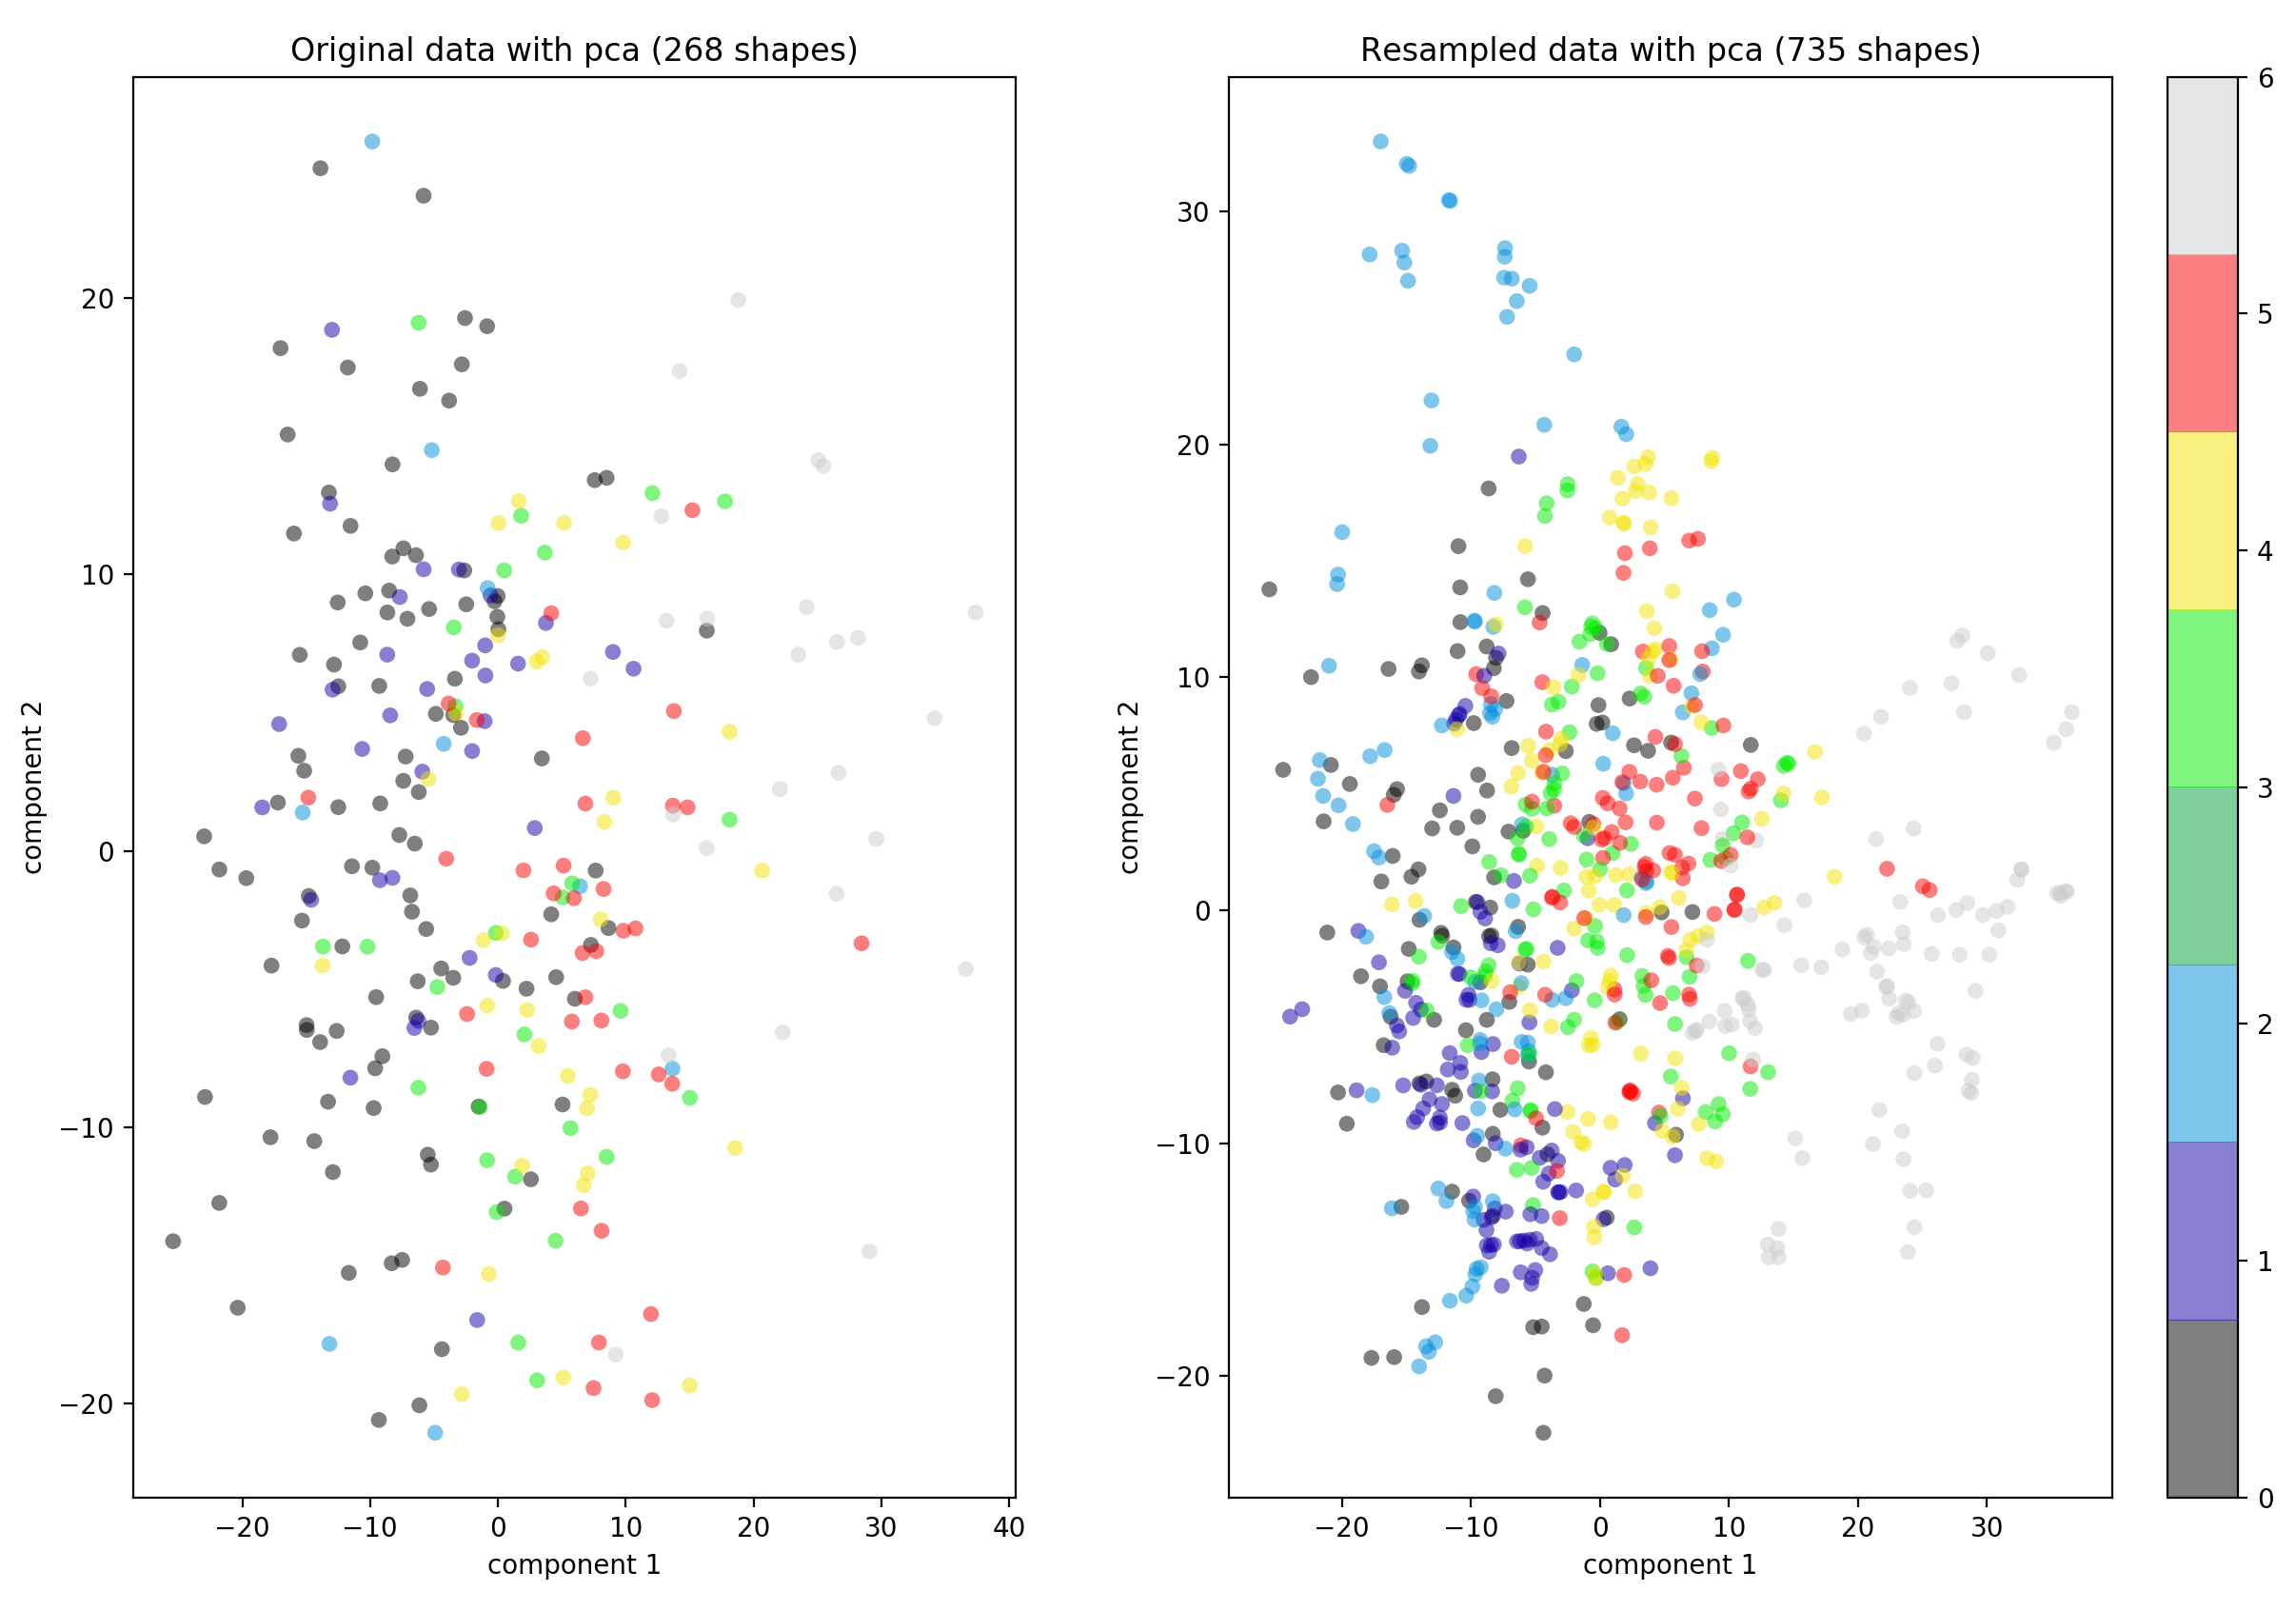
\includegraphics[width=0.95\textwidth]{SMOTE_resample.png}}
    \caption{After resampling with SMOTE, each group has 105 data points.}
    \label{fig:SMOTEresample}
\end{figure}
Figure \ref{fig:SMOTEresample} shows the first two principal components plotted
before and after SMOTE resampling. After SMOTE, each class has 105 data points
and is now suitable to train a neural network. 
The next section will show the results of training and classification of our neural network. 

\section{RESULTS}

The neural network has 4 hidden layers with [4096, 2048, 1024, 512] neurons, a drop out layer with probability $0.5$ and 
softmax layer with 7 outputs. The learning rate was set to $1^{-5}$. The network was trained for 100 epochs and the batch size was set to $32$.
\begin{figure}[h]
\centering 
    \subfigure[Cross entropy loss]{\label{fig:crossentropy}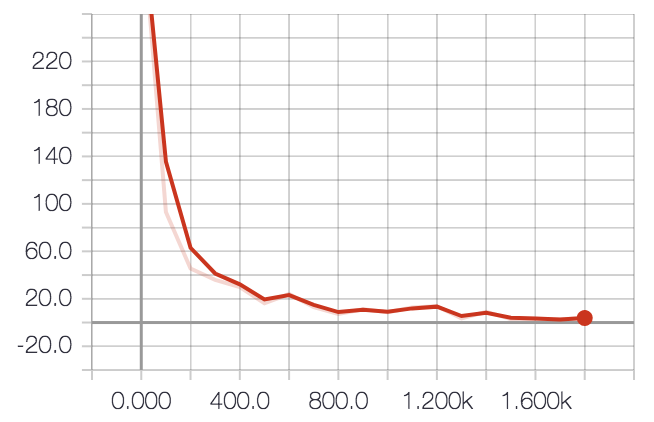
\includegraphics[width=0.45\textwidth]{cross_entropy.png}}
    \subfigure[Accuracy]{\label{fig:accuracy}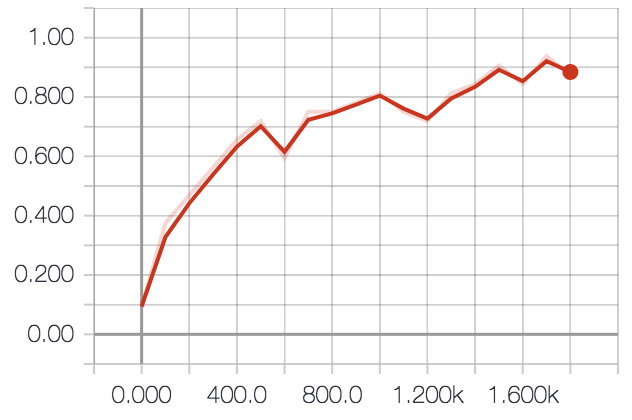
\includegraphics[width=0.45\textwidth]{accuracy.png}}
    \caption{Cross entropy loss function and accuracy during training.}
    \label{fig:learning}
\end{figure}
The SVA training is shown in Figure \ref{fig:learning}.
The maximum accuracy during training was $93\%$. 
The dataset was subdivided in two sets, training and testing in a $80/20$ ratio. 
The testing data was not used at any point during training and it 
will be used to test if the trained network generalizes well for unseen data samples. 
Using the testing dataset, the accuracy achieved was $95\%$. 

% The SVA performance is shown in the confusion matrix \ref{tab:confusion}, 
% where each column represents the instances in the SVA classification group,
% while each row represents the group instances as assessed by the consensus between two clinician experts. 
% Agreement between the clinician consensus and the SVA classification are located in the main diagonal of the table. 
% Cells adjacent to the main diagonal (1 diagonal 
% to the right and 1 diagonal to the left) indicate the classification of the degree of degeneration was within 1 group difference. The main and adjacent diagonals include 91\% of the testing dataset. 
% The cells outside the 3 middle diagonals show that 3 out of 34 condyles were classified with 2 or more groups difference. 

% \begin{table}[]
% \centering
% \caption{Confusion matrix: columns show the SVA classification of condylar morphology; rows show the clinician experts consensus classification. The main diagonal cells show when the group was classified by the SVA exactly the same as the clinicians. The cells in 1 diagonal to the right and 1 diagonal to the left show number of condyles where the prediction differed from clinicians by only one group and still indicates an acceptable estimate of severity/risk level of disease staging. A challenge is that clinician expert assessment is limited by their visual perception of the 3D morphology. Note that as the testing dataset is from patients with less than 5 years of  diagnosis of the disease, SVA  did not classify any  group 4 or  5 of  more  advanced disease stag in the testing sample, as expected.in such disease  condition that  the degeneration progresses in a chronic process through many years. }
% \label{tab:confusion}
% \begin{tabular}{lllllll}
% ClinE \textbackslash  SVA & 01 & 02 & 03 & 04  & 05 & 06 \\
% 01                       & 1 & 0 & 0 & 0  & 0 & 0 \\
% 02                       & 7 & 1 & 0 & 0  & 0 & 0 \\
% 03                       & 2 & 2 & 1 & 4  & 0 & 0 \\
% 04                       & 1 & 0 & 1 & 10 & 0 & 0 \\
% 05                       & 0 & 0 & 0 & 2  & 2 & 0 \\
% 06                       & 0 & 0 & 0 & 0  & 0 & 0
% \end{tabular}
% \end{table}

\section{CONCLUSION}

SVA is new tool to analyze shape variation using deep neural networks. 
The results presented here indicate that using shape features only favors the classification task, i.e., 
we do not include any information about position or orientation of the model. 
This classification approach seems promising, as it may help us increase our understanding about 
shape changes that TMJ OA patients undergo during the course of the disease. 
The source code repository is available at \url{https://github.com/DCBIA-OrthoLab/ShapeVariationAnalyzer}

Future work will focus on including additional predictors/features of the disease in
the neural network training (e.g., clinical data, behavioral or biochemical). 
Clinical and behavioral data has been acquired through questionnaires, while biochemical 
data has been acquired through a protein analysis in saliva and plasma samples.
Including these may contribute to improve the classification power of the neural network.


%%%%%%%%%%%%%%%%%%%%%%%%%%%%%%%%%%%%%%%%%%%%%%%%%%%%%%%%%%%%%
%%%%% References %%%%%
\bibliography{report}   %>>>> bibliography data in report.bib
\bibliographystyle{spiebib}   %>>>> makes bibtex use spiebib.bst

\end{document} 
